%!TEX root = ../StatisticalCorrelations.tex

\graphicspath{{Body/Figures/EvW/}{Body/Figures/GoodnessOfFit/}}

\section{Monte Carlo}


In order to determine correlation coefficients between the various analyses, a Monte Carlo simulation was developed. This Monte Carlo generates pseudo-data according to the different analysis types, fills histograms defined by the parameters in \tabref{tab:analyzerParameters}, and then fits them accordingly. Pseudo-data was generated using \ROOT's \texttt{TF2->GetRandom2()} method. The 2D function used to generate the data is given by a five parameter function with energy dependence on the number, asymmetry, and phase terms,
\begin{align}
	N(t, E) = N_{0}(E) \cdot e^{-t/\tau_{\mu}} \cdot (1 + A(E) \cos{(\omega_{a}t + \phi(E))}),
\label{eq:2dfunc}
\end{align}
with the time-dilated muon lifetime \taumu equal to \ns{64440} and \gmtwo frequency \wa set as
\begin{align}
	\omega_{a} = 2\pi \cdot 0.2291 \text{MHz} \cdot (1 + R \times 10^{-6}),
\end{align}
where \R was set to 0. 


\subsection{Function Input}


The energy dependent terms in \equref{eq:2dfunc} were determined from energy-binned fits to the data provided by D. Sweigart for ReconEast and M. Sorbara for ReconWest, for each of the four datasets in \Rone. \figref{fig:energyBinFits} show the respective histograms for the 9d dataset, where it can be seen that energy bin fits to the two reconstructions produce very similar histograms. The \RE energy bin fits ranged from \SIrange{300}{3100}{\MeV} in bins of \SI{50}{\MeV} for a total of 56 energy bins, while the \RW energy bin fits ranged from \SIrange{300}{3060}{\MeV} in bins of \SI{60}{\MeV} for a total of 46 energy bins. Two \texttt{TF2}s were constructed using either the \RE or \RW histograms as input. The number of Y points in the functions were set as the number of bins in the respective histograms, and the function was defined such that the energy binned histograms would be linearly interpolated between the values at the bin centers. The number of X points in the functions were defined such that the function ranged from \SIrange{0}{699971.8}{ns} in steps of $149.2/2 = 74.6 \text{ns}$ for a total of 9383 points. This `point-width' was chosen for a couple of reasons. The first is that the maximum number of allowed X or Y points in a \texttt{TF2} is 10000, and this point-width results in a number of points close to but not above that value. The second is that it is either exactly or very close to a multiple of the bin widths chosen by the analyzers. It was found that using the maximum number of points such that the point width was \ns{70} (for a range up to \ns{700000}) resulted in aliasing frequencies appearing in the generated data. With a point-width of \ns{74.6} these aliasing frequencies disappeared entirely except in some Q-Method fits, as evidenced by the non-flat p-value distribution in \figref{}. In order to remove this issue entirely a different implementation beyond \texttt{TF2} would be needed. The 2D function parameters are summarized in \tabref{tab:2dfunctionParameters}.



\begin{figure}[]
\centering
    \begin{subfigure}[t]{0.45\textwidth}
        \centering
        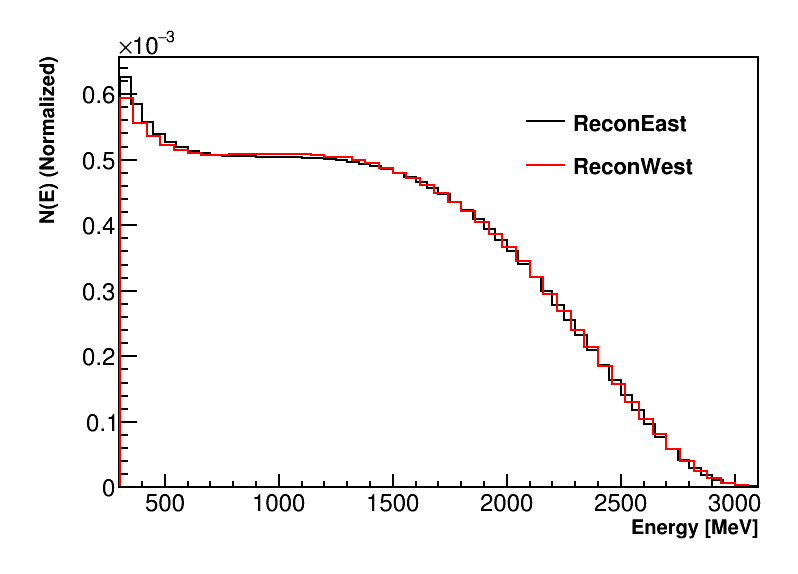
\includegraphics[width=\textwidth]{ReconEastvWest_N}
        \caption{$N(E)$}
    \end{subfigure}% %you need this % here to add spacing between subfigures

    \begin{subfigure}[t]{0.45\textwidth}
        \centering
        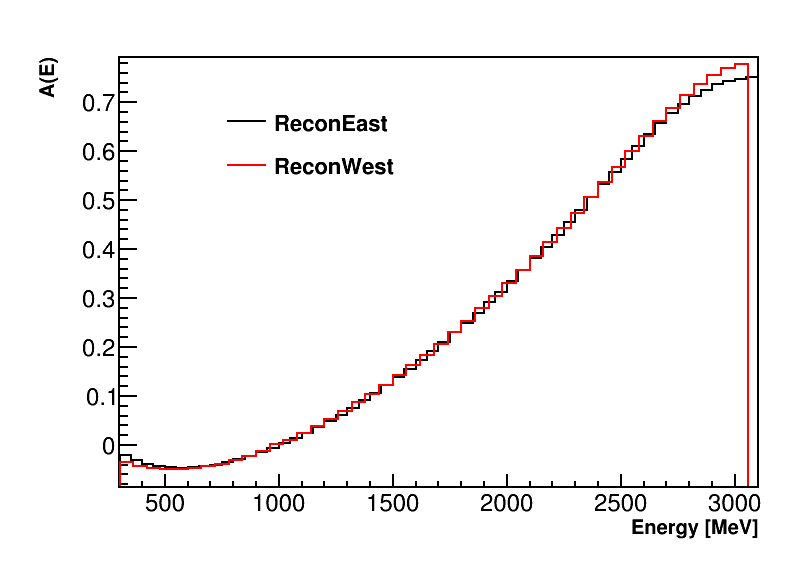
\includegraphics[width=\textwidth]{ReconEastvWest_A}
        \caption{$A(E)$}
    \end{subfigure}
    \hspace{1mm}
    \begin{subfigure}[t]{0.45\textwidth}
        \centering
        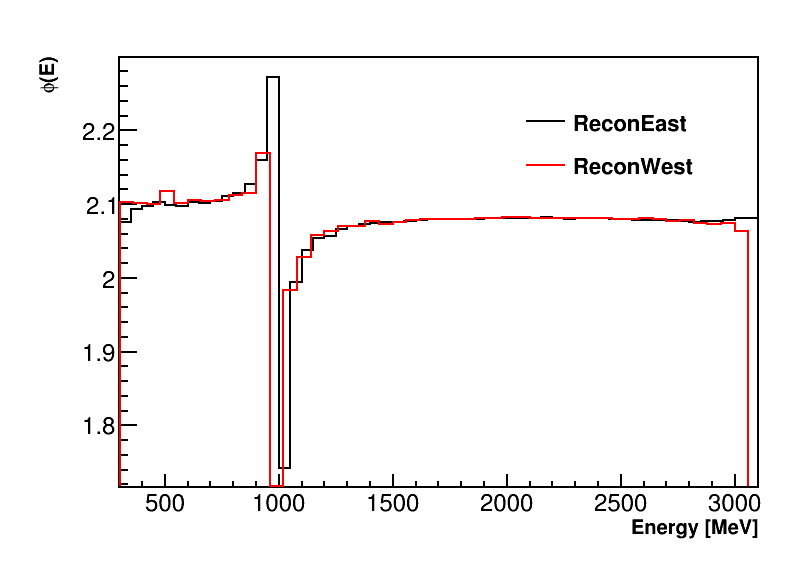
\includegraphics[width=\textwidth]{ReconEastvWest_Phi}
        \caption{$\phi(E)$}
    \end{subfigure}
\caption[]{$N$, $A$, and $\phi$ as a function of energy from energy bin fits to \RE (black) and \RW (red) data for the 9d dataset. These histograms are representative of the quantities for all datasets, though there are slight differences. The \RE energy bin fits ranged from \SIrange{300}{3100}{\MeV} in bins of \SI{50}{\MeV} for a total of 56 energy bins, while the \RW energy bin fits ranged from \SIrange{300}{3060}{\MeV} in bins of \SI{60}{\MeV} for a total of 46 energy bins, hence the different bin edges in the plot. There are some slight differences at low and high energies within the various plots, but for the most part the two reconstructions behave very similary.}
\label{fig:energyBinFits}
\end{figure}



\begin{table}
\centering
\renewcommand{\arraystretch}{1.2}
\begin{tabularx}{1\linewidth}{@{\extracolsep{\fill}}lcc}
  \hline
    \multicolumn{3}{c}{\textbf{2D Function Parameters}} \\
  \hline\hline
     & \thead{\RE Input} & \thead{\RW Input} \\
  \hline
  	Energy Range (\MeV) & 300--3100 & 300--3060 \\
  	Energy Points & 56 & 46 \\ 
  	Energy Point-Width (\MeV) & 50 & 60 \\
  	Time Range (ns) & 0--699971.8 & 0--699971.8 \\
  	Time Points & 9383 & 9383 \\
  	Time Point-Width (ns) & 74.6 & 74.6 \\
  \hline
\end{tabularx}
\caption[]{Parameters used to define the \texttt{TF2}s in the Monte Carlo pseudo-data generation.}
\label{tab:2dfunctionParameters}
\end{table}



\subsection{\RE vs \RW}

The \texttt{TF2}s take input from either \RE or \RW energy bin functions as described previously. In order to properly estimate correlation coefficients including the effects of the reconstructions, a comparison between \RE and \RW is necessary. J. LaBounty studied the different reconstructions of clusters in detail \cite{JoshEvW}. In doing so he determined that the cluster times between the two reconstructions were the same to high precision, but that there were differences in the reconstructed cluster energies. He took \RE and \RW analyses, isolated produced clusters from the same waveforms, and plotted the energies against each other. The calorimeter sum of this comparison for the 9d dataset is shown in \figref{fig:EvWenergies}. As shown most hits lie along the unit slope line. Some hits off in different bands either due to reconstruction differences or some individual crystals which had poor relative energy calibration. Taking projections of this distribution, energies can be converted between \RE and \RW by sampling those projections. An example is given in \figref{fig:EvWprojection}.


A couple of points should be mentioned. First is that the bin width used by J. LaBounty was \SI{10}{\MeV}, certainly discrete enough for the purposed of this Monte Carlo and also finer than the energy bin widths used in the generation of the \texttt{TF2}s. Second is that the comparison is built upon clusters before they have been corrected for pileup, hence the counts out at energies beyond the magic momentum of \SI{3.094}{\GeV} plus the energy resolution. It is expected that this should be fine to use since pileup is a minimal effect and should effect \RE and \RW more or less equally. Third is that this comparison was built upon D. Sweigart's and A. Fienberg's analyses. D. Sweigart is the only \RE analyzer, while A. Fienberg was one of several \RW analyzers. Since A. Fienberg uses different clustering parameters than the rest of the \RW analyzers, (\texttt{timeCutoffLow = 2, timeCutoffHigh = 3} vs \texttt{timeCutoffLow = 3, timeCutoffHigh = 5}), the comparison isn't apples to apples. It is mentioned that for the most technically correct results the \RE vs \RW comparison should be done individually for all analyzers, though the final results are not expected to change significantly.



\begin{figure}[]
\centering
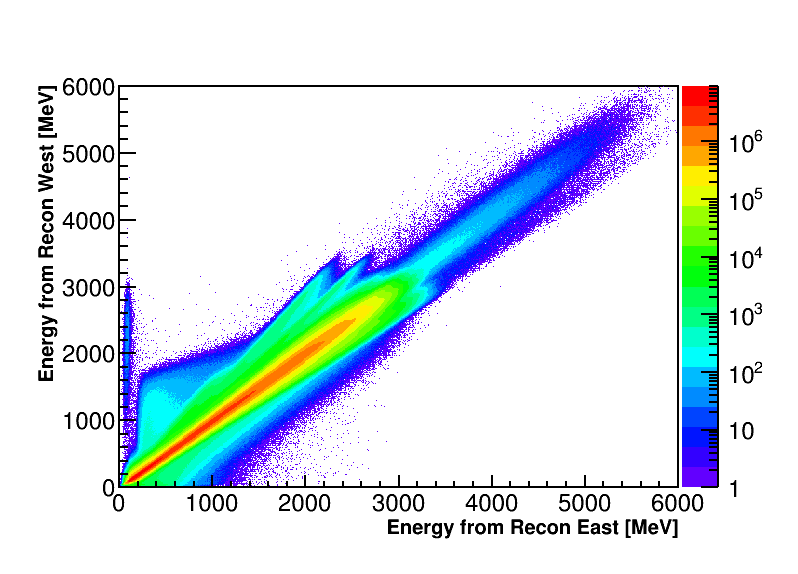
\includegraphics[width=.7\textwidth]{ReconEastvWest_Energies}
\caption{Log-scale plot of \RE energies vs \RW energies for the same produced clusters for the 9d dataset. The plot shows that the large majority of hits form a Gaussian around the unit slope line, however there are bands of hits outside this line due to effects such as some individual crystals in some calorimeters with poor energy calibration. This pattern was determined to be stable throughout the fill. \RE vs \RW comparison performed by J. LaBounty \cite{JoshEvW}. }
\label{fig:EvWenergies}
\end{figure}

\begin{figure}[]
\centering
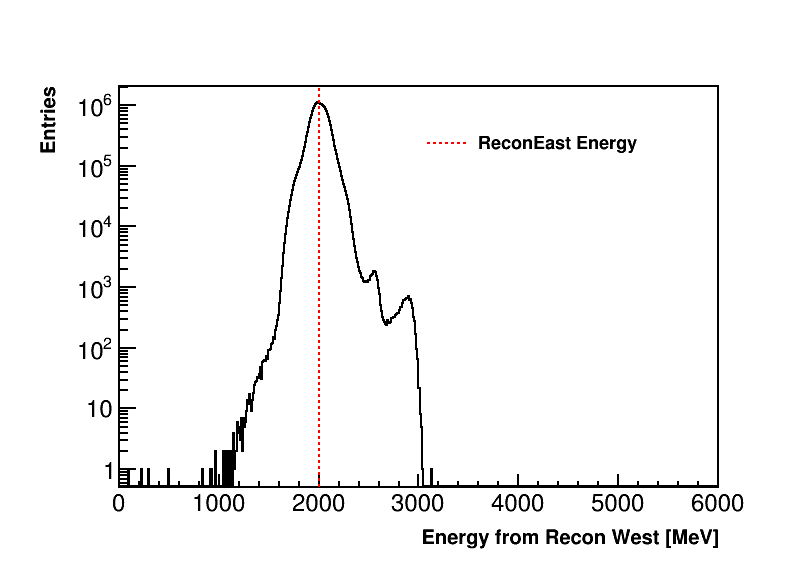
\includegraphics[width=.7\textwidth]{ReconEastvWest_Projection}
\caption{A Y-axis or \RW energy projection for a chosen \RE energy of \SI{2}{\GeV}. The plot is on a log-scale, with a mainly Gaussian structure. Tails and peaks due to the banding structure can be seen however.}
\label{fig:EvWprojection}
\end{figure}




\subsection{Event Generation and Randomization}


Events were generated through \texttt{TF2->GetRandom2()} method calls. Many samples of pseudo-data were generated via the same procedure, for each dataset and for the two \texttt{TF2} variants with input from either \RE or \RW. The number of hits per dataset was determined empirically such that the error on the fitted \R value is comparable to the \Rone datasets, where the approximate level of statistics for the 60h, HK, 9d, and EG datasets are given by \{5.04e9, 7.01e9, 1.08e10, 2.21e10\}. (These numbers depend on the energy and time ranges of the \texttt{TF2}s and hence do not correspond directly to the real dataset statistics, what's important and what is replicated is the number of hits which end up in the wiggle plot within the fit ranges.) The errors on \R were always within \SIrange{10}{20}{ppb} of the actual analysis values (and many times within \ppb{1}).

Note that in the event generation no time-randomization was included, as is done by the analyzers in order to remove effects of the fast rotation. It is expected that in the Monte Carlo with no fast rotation effect, with enough random seeds, the mean \R value is equivalent to the non-time-randomized \R value. While the spread in the \R values will be slightly less without the time-randomization, this is expected to negligibly affect the final correlation coefficients. This effect could be included at the expense of many CPU hours since the event generation would take significantly longer.

The procedure for the event generation is as follows:
\begin{enumerate}
	\item{A number of hits per sample and per dataset is determined via \texttt{PoissonD()} method calls on the static number of statistics per dataset such that each sample has a very slightly different amount of statistics.} 
	\item{For each hit or entry, \texttt{TF2->GetRandom2()} is called on one of the two 2D input functions to generate a time or energy.}
	\item{The hit energies are designated either as \RE or \RW. For either variant, the corresponding \RW or \RE energy is determined by randomly sampling the corresponding energy projection as determined from J. LaBounty's studies, see \figref{fig:EvWprojection}. This projection is sampled via \texttt{TH1->GetRandom()} method calls. Whatever the first generated energy is, \RE or \RW, is also designated as the Q-Method energy.}
	\item{The corresponding energies, asymmetries, and weights are then used to fill histograms defined by the analyzer parameters given in \tabref{tab:analyzerParameters}.}
	\item{Because the R-Method has intrinsic randomization in how the counts get put into the four Ratio histograms, these Ratio histograms are produced for 100 random seeds. The randomization of counts is performed via \texttt{GetUniform()} method calls.} 
\end{enumerate}


In all instances of the randomization, including the randomization on the number of events, sampling the \texttt{TF2}s, sampling the \RE vs \RW energy projections, and the ratio randomization, the \ROOT\texttt{TRandomMixMax} class is used. The standard \texttt{TRandom3} class was initially used and found to be inadequate for this high precision statistical study. \texttt{TRandomMixMax} has the advantage of producing proper random numbers with high periodicity, and also being fast enough to produce the high numbers of needed events in a reasonable time frame\footnote{This generator is the default used in Geant4.}\cite{TRandom}.


-talk about submitting jobs to the grid here or elsewhere? 



\subsection{Fitting the Pseudo-Data}

- need to mention which fitting ranges I'm using, for EG and all that, point back to first table


Once the pseudo-data has been generated, the data is fit either with a simple five parameter function in the TAQ-Methods,
\begin{align}
    N(t) = N_{0} \cdot e^{-t/\tau_{\mu}} \cdot (1 + A \cos{(\omega_{a}t + \phi})),
\label{eq:fiveParFit}
\end{align}
or a simple three parameter function in the case of the R-Method,
\begin{align}
    R(t) =A \cos{(\omega_{a}t + \phi}).
\label{eq:ratioFit}
\end{align}
In both cases the energy dependent pieces from \equref{eq:2dfunc} are gone, and the fitted constants will converge to their integrated values. \figref{fig:sampleFits} shows examples of fits to the four different methods, for the same generated sample. In general the fit parameters are very similar to one another between the different methods, however due to the different analyzer parameters chosen like energy threshold, the fit parameters can be slightly, but significantly, different. \figref{fig:FFTs} shows the FFTs of the fits from \figref{fig:sampleFits}. What can sometimes occur, though isn't shown here, is that aliasing peaks can appear at beat frequencies with \wa, due to differences in the point-width frequency of the input 2D function and the bin width of the histogram. Once the order-1000 grid jobs are submitted and the histograms are returned, all the samples and all the seeds are fit. The fit parameters are stored into \ROOT trees so that the parameters for the different methods and samples can be compared. 

Similarly, measures of the goodness-of-fit are also stored, in order to verify that the pseudo-data is being fit correctly. P value distributions for the four methods for one set of grid jobs is shown in \figref{fig:pValues}. As shown the distributions are flat for the TA-Methods, and are not flat for the RQ-Methods. The Q-Method is understood to be non-flat due to the difference in bin width and point-width mentioned previously, while the origin of the non-flatness of the R-Method is unkwown at this time. \figref{fig:pulls} show the pulls on \R for the different samples in this set of submitted grid jobs. The distributions in general are very close to unit-Gaussians, with some slight deviations in the RQ-Method cases leading to slight pulls on \R. This should have a very minimal effect on the calculated correlation coefficients, but it should be kept in mind.


\begin{figure}[]
\centering
    \begin{subfigure}[t]{0.45\textwidth}
        \centering
        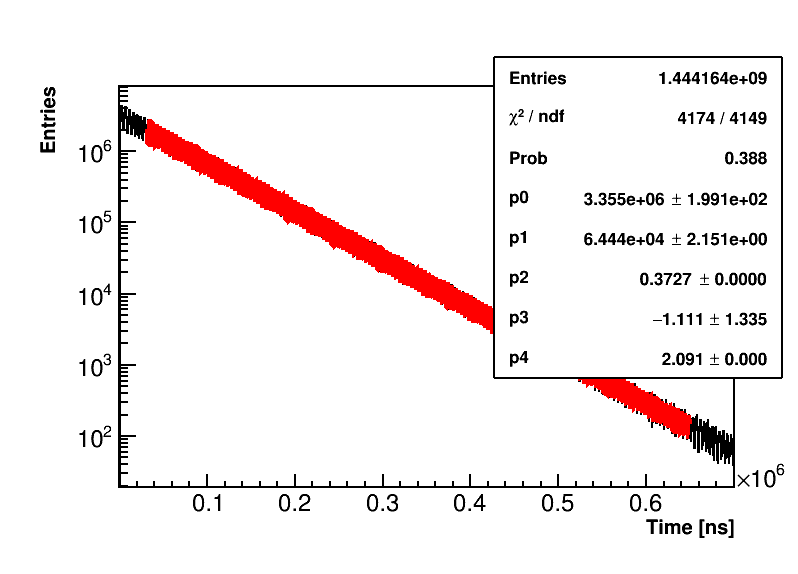
\includegraphics[width=\textwidth]{Example_TMethod_Fit}
        \caption{T-Method}
    \end{subfigure}
    \hspace{1mm}
    \begin{subfigure}[t]{0.45\textwidth}
        \centering
        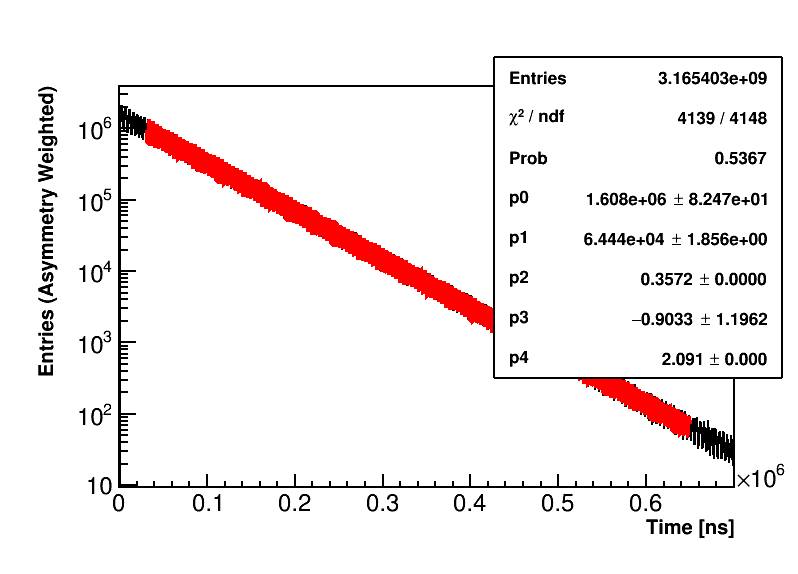
\includegraphics[width=\textwidth]{Example_AMethod_Fit}
        \caption{A-Method}
    \end{subfigure}% %you need this % here to add spacing between subfigures

    \begin{subfigure}[t]{0.45\textwidth}
        \centering
        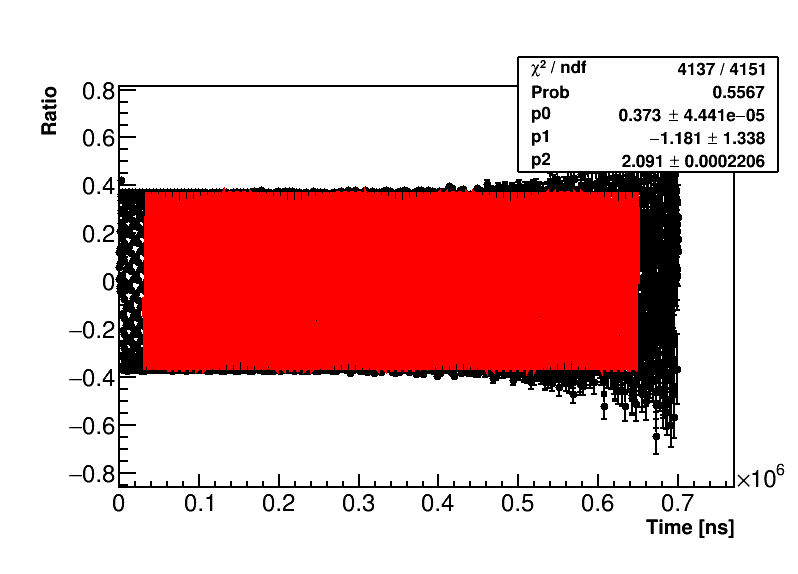
\includegraphics[width=\textwidth]{Example_RMethod_Fit}
        \caption{R-Method}
    \end{subfigure}
    \hspace{1mm}
    \begin{subfigure}[t]{0.45\textwidth}
        \centering
        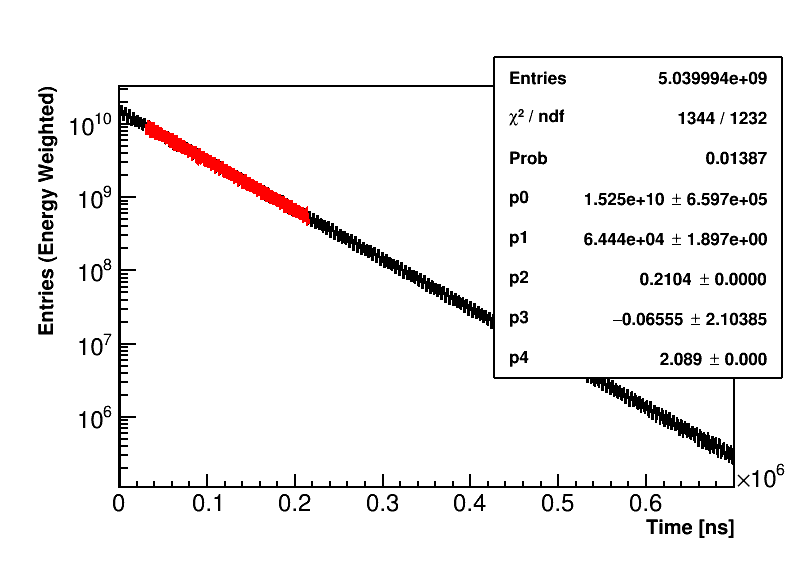
\includegraphics[width=\textwidth]{Example_QMethod_Fit}
        \caption{Q-Method}
    \end{subfigure}
\caption[]{TARQ-Method fits to a sample generated from the 60h functions.}
\label{fig:sampleFits}
\end{figure}
%-T method was from Aaron, A method from David, R method from me, and Q from Tim


\begin{figure}[]
\centering
    \begin{subfigure}[t]{0.45\textwidth}
        \centering
        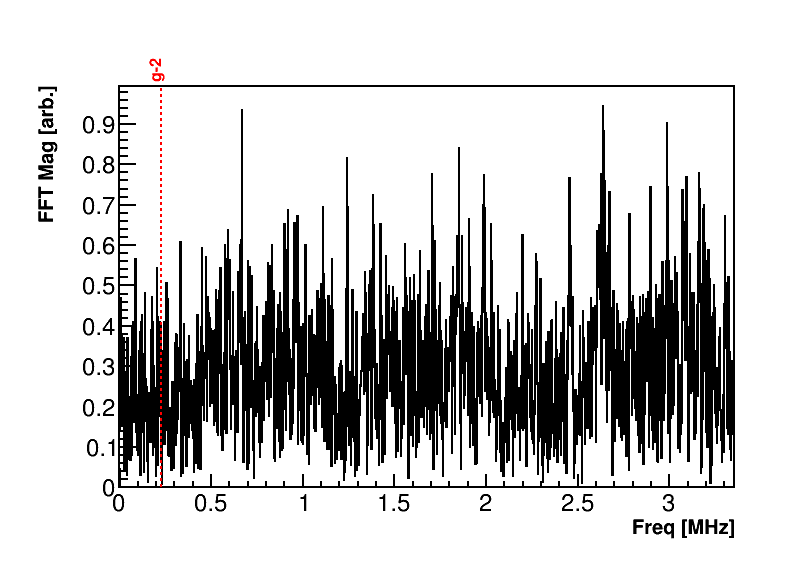
\includegraphics[width=\textwidth]{FFT_TMethod}
        \caption{T-Method}
    \end{subfigure}
    \hspace{1mm}
    \begin{subfigure}[t]{0.45\textwidth}
        \centering
        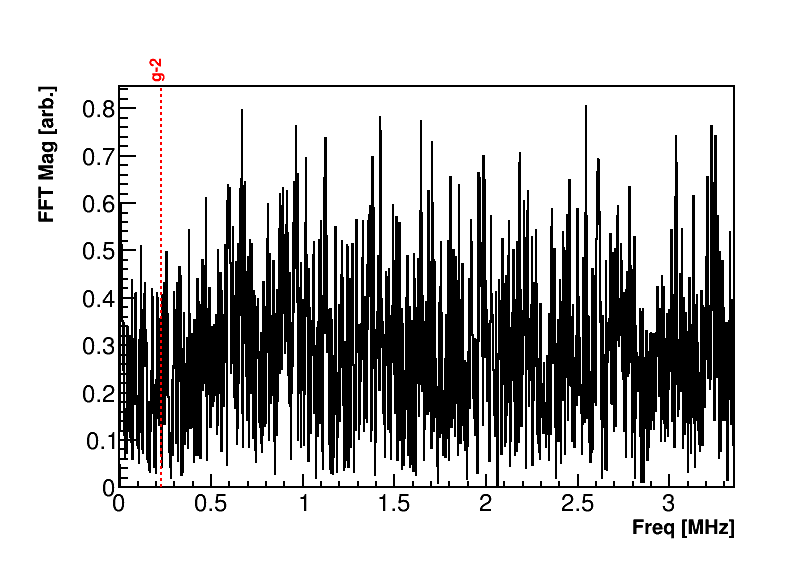
\includegraphics[width=\textwidth]{FFT_AMethod}
        \caption{A-Method}
    \end{subfigure}% %you need this % here to add spacing between subfigures

    \begin{subfigure}[t]{0.45\textwidth}
        \centering
        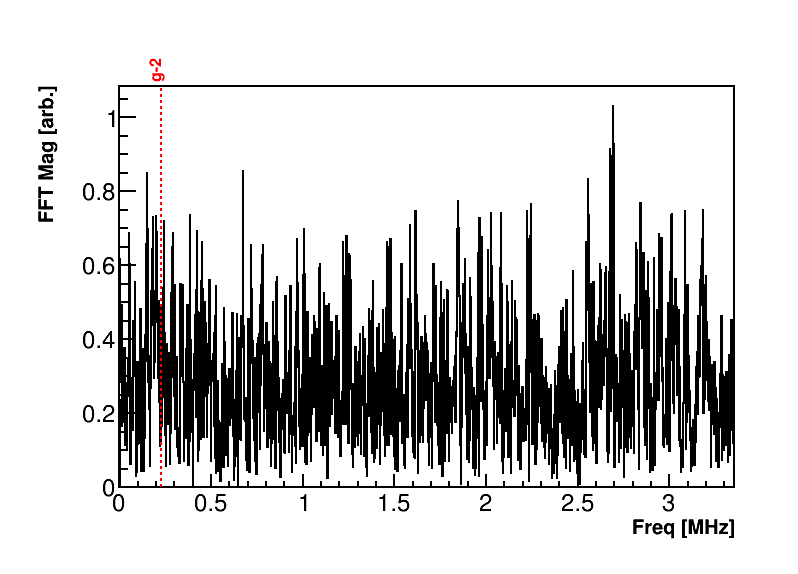
\includegraphics[width=\textwidth]{FFT_RMethod}
        \caption{R-Method}
    \end{subfigure}
    \hspace{1mm}
    \begin{subfigure}[t]{0.45\textwidth}
        \centering
        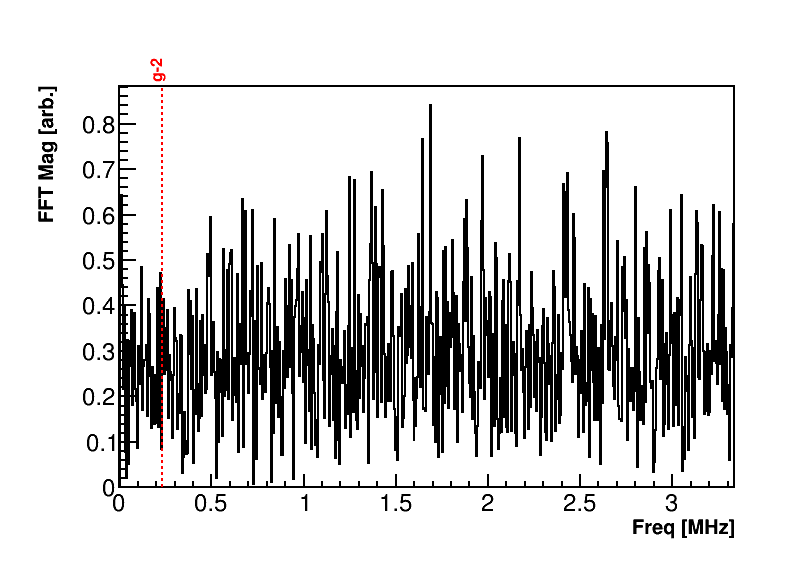
\includegraphics[width=\textwidth]{FFT_QMethod}
        \caption{Q-Method}
    \end{subfigure}
\caption[]{FFTs of the TARQ fits shown in \figref{fig:sampleFits}.}
\label{fig:FFTs}
\end{figure}


\begin{figure}[]
\centering
    \begin{subfigure}[t]{0.45\textwidth}
        \centering
        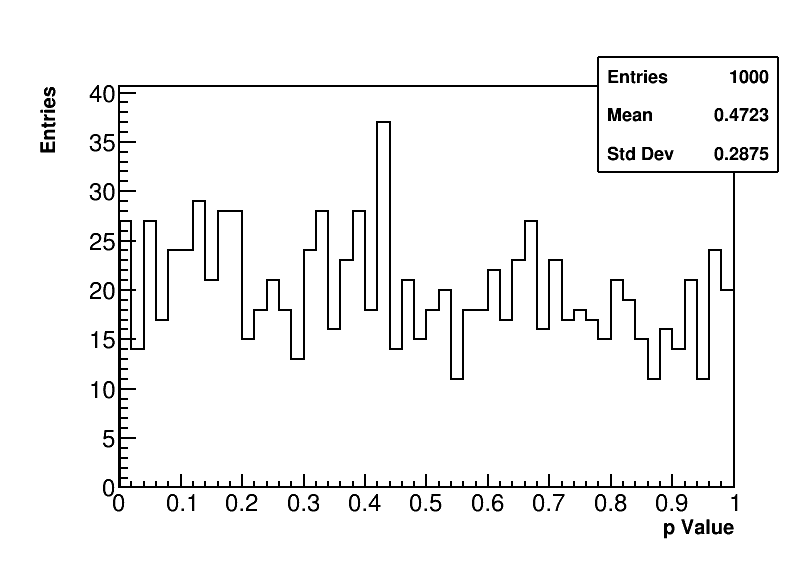
\includegraphics[width=\textwidth]{PValues_TMethod}
        \caption{T-Method}
    \end{subfigure}
    \hspace{1mm}
    \begin{subfigure}[t]{0.45\textwidth}
        \centering
        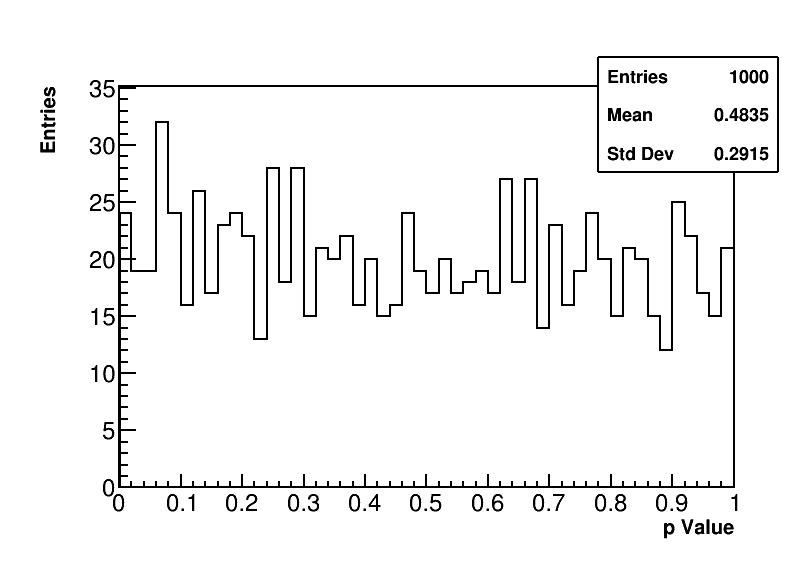
\includegraphics[width=\textwidth]{PValues_AMethod}
        \caption{A-Method}
    \end{subfigure}% %you need this % here to add spacing between subfigures

    \begin{subfigure}[t]{0.45\textwidth}
        \centering
        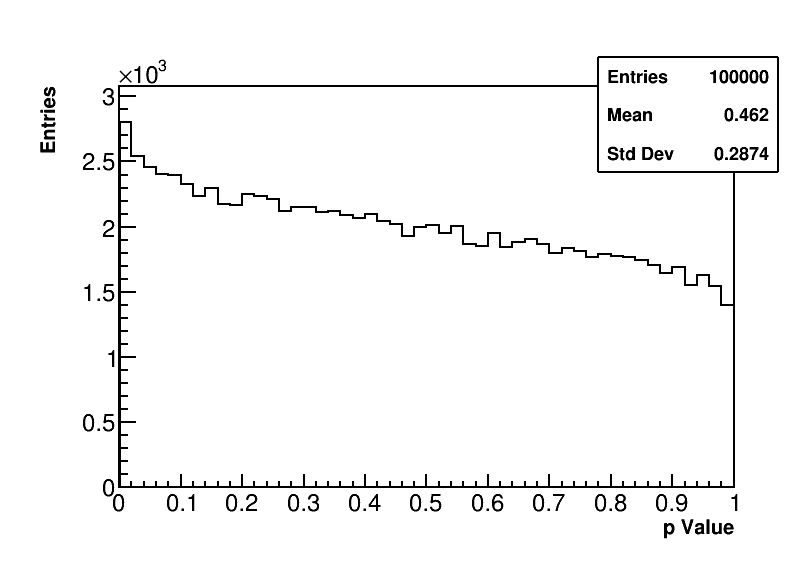
\includegraphics[width=\textwidth]{PValues_RMethod}
        \caption{R-Method}
    \end{subfigure}
    \hspace{1mm}
    \begin{subfigure}[t]{0.45\textwidth}
        \centering
        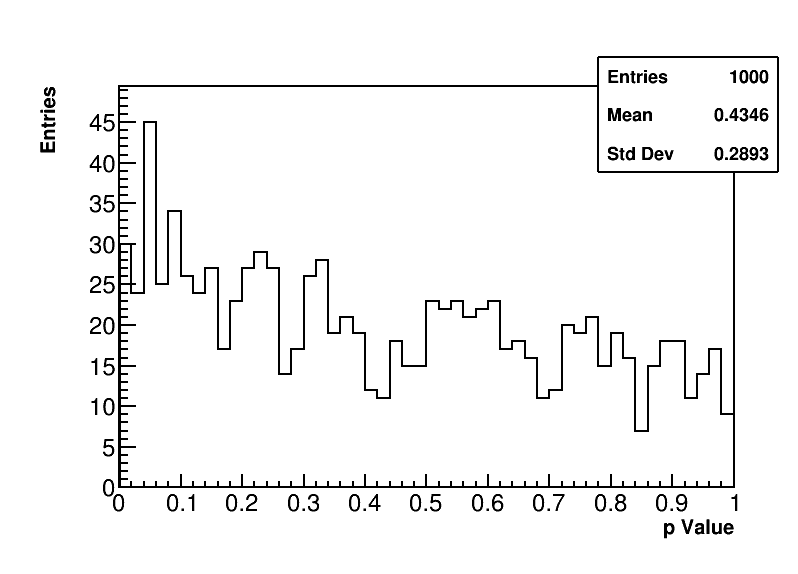
\includegraphics[width=\textwidth]{PValues_QMethod}
        \caption{Q-Method}
    \end{subfigure}
\caption[]{P-value distributions for one submission of grid jobs, hence the 1000 entries in the TAQ-Method plots, and the 1000 entries times 100 random seeds for the R-Method plot. The TA-Method p values are flat, while the RQ-Method p values are not. In the case of the Q-Method, the non-flat shape can be attributed to the difference in bin width and 2D function point-width. The origin of the non-flat shape for the R-Method is unknown at this time.}
\label{fig:pValues}
\end{figure}


\begin{figure}[]
\centering
    \begin{subfigure}[t]{0.45\textwidth}
        \centering
        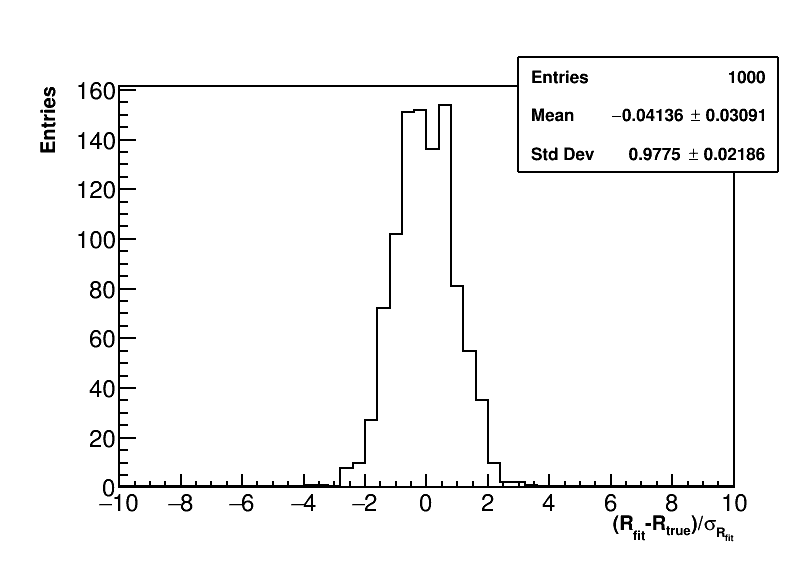
\includegraphics[width=\textwidth]{Rpull_TMethod}
        \caption{T-Method}
    \end{subfigure}
    \hspace{1mm}
    \begin{subfigure}[t]{0.45\textwidth}
        \centering
        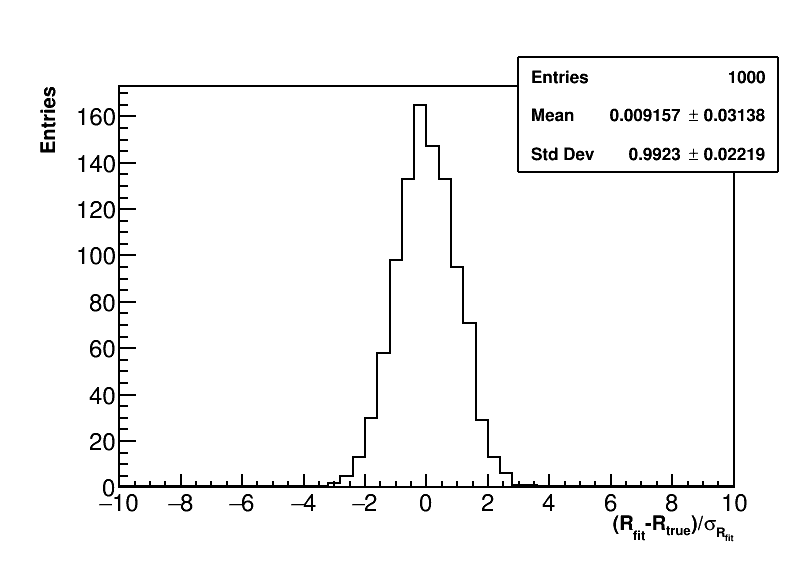
\includegraphics[width=\textwidth]{Rpull_AMethod}
        \caption{A-Method}
    \end{subfigure}% %you need this % here to add spacing between subfigures

    \begin{subfigure}[t]{0.45\textwidth}
        \centering
        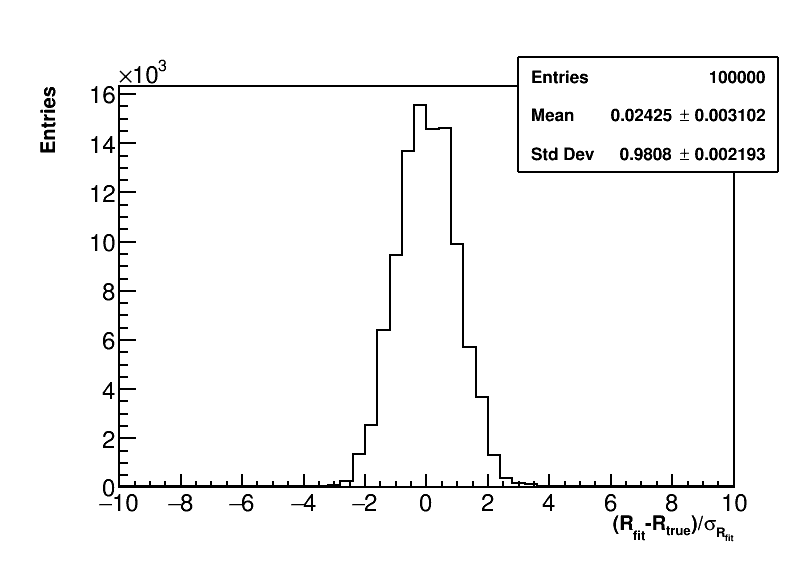
\includegraphics[width=\textwidth]{Rpull_RMethod}
        \caption{R-Method}
    \end{subfigure}
    \hspace{1mm}
    \begin{subfigure}[t]{0.45\textwidth}
        \centering
        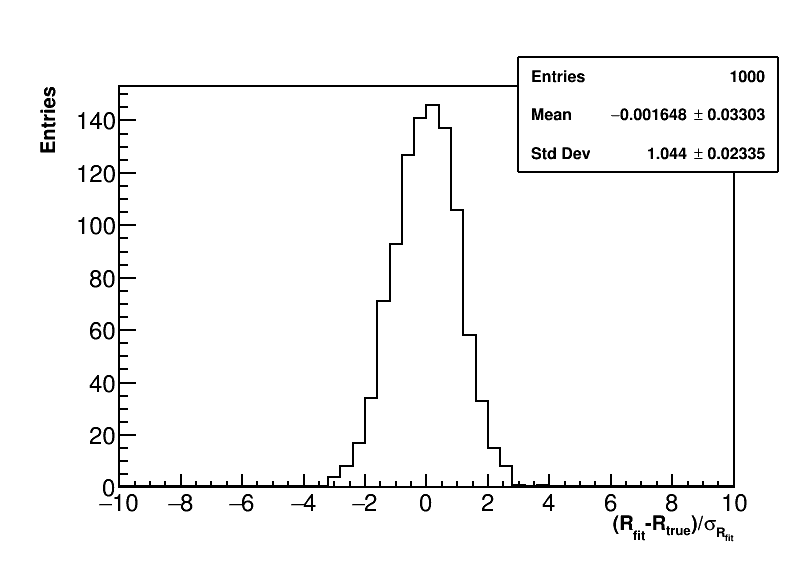
\includegraphics[width=\textwidth]{Rpull_QMethod}
        \caption{Q-Method}
    \end{subfigure}
\caption[]{Pulls for the TARQ-Methods. The various distributions are close to unit-Gaussians, with differences in some RQ-Method cases which again is attributed to imperfect fits.}
\label{fig:pulls}
\end{figure}




% - don't do pileup, the effect should be a lot smaller than the energy threshold changes between analyses after pileup subtraction, it would be a major effort to somehow put in different pileup cases, etc.

